\chapter{Ion trapping with {$^{40}$Ca$^+$}}

In this section we discuss the fundamental theory and principles of trapping and manipulating $^{40}$Ca$^+$ ions, which were used in all of the experiments described in this thesis. First we will discuss the fundamental principles of radio frequency (RF) traps which lead to approximately harmonic trapping potentials. We will then describe the characteristics and spectroscopy the of $^{40}$Ca$^+$ ion, the theory of laser-ion interactions, and other relevant experimental details that pertain to the state manipulation and measurement of this ion. 


%%%%%%%%%%%%%%%%%%%%%%%%%%%%%%%%%%%%%%%%%%%%%%%%%%%%%

\section{Radio frequency trap principles and ion dynamics}

A thorough review of ion trapping in radio frequency traps can be found in Refs. \cite{Wineland98.NIST.103.259, Leibfried03.RMP.75.281, Häffner2008155, Roos00.Thesis}. Here we will review the essential principles, as well as the resulting ion dynamics, that are relevant to our experiments. We assume that the ions will be trapped by a quadrupolar potential that can, near its center, be decomposed into static (DC) and sinusoidally varying (RF) components:
\begin{equation} 
\Phi (\textbf{r}, t) = \frac{U}{2} ( \alpha_x \ x^2 + \alpha_y \ y^2 + \alpha_z \ z^2 ) + \frac{V_{RF} \cos{(\Omega_{RF} t)}}{2} ( \alpha'_x \ x^2 + \alpha_y \ y^2 + \alpha_z \ z^2 ) \text{.}
\end{equation}
In our configuration we use an RF drive frequency $\approx$ 50 MHz. The geometric factors $\alpha_i$ and $\alpha'_i$ depend on the trap design and must satisfy the Laplace equation $\nabla^2 \Phi = 0$. In a linear trap configuration, the RF potential provides dynamic radial confinement in two radial dimensions while static potentials provide axial confinement in the third dimension. Choosing $z$ as our axial coordinate, we can use $\alpha_x + \alpha_y = - \alpha_z$, $\alpha'_x = - \alpha'_y$, and $\alpha'_z = 0$, which satisfies the Laplace equation. 

The classical equation of motion for a particle with charge $Q$ and mass $m$ is
\begin{equation}
\ddot{u} = - \frac{Q}{m} \frac{\partial \Phi}{\partial u} = - \frac{Q}{m} [ U \alpha_u + V_{RF}\cos{(\Omega_{RF} t)} \alpha'_u ] \ u
\end{equation}
and can be transformed into the canonical form of the Mathieu equation 
\begin{equation}
\frac{\partial^2 u}{\partial \xi^2} + [ a_u + 2 q_u \cos{(2 \xi)} ] \ u = 0 
\end{equation}
by the substitutions
\begin{equation}
\xi = \frac{1}{2} \Omega_{RF} \ t \text{,} \ \ \ \ \ \ \ \ a_u = \frac{4 Q U \alpha_u}{m \Omega_{RF}^2} \text{,} \ \ \ \ \ \ \ \ q_u = \frac{2 Q V_{RF} \ \alpha'_u}{m \Omega_{RF}^2} \ \text{.}
\end{equation}
Therefore, in the linear trap configuration the equations of motion near the center/null of the RF potential become
\begin{equation}
\begin{split}
\frac{\partial^2 x}{\partial \xi^2} + [ a_x + 2 q_x \cos{(2 \xi)} ] \ x = 0  \\
\frac{\partial^2 y}{\partial \xi^2} + [ a_y + 2 q_y \cos{(2 \xi)} ] \ y = 0  \\
\frac{\partial^2 x}{\partial \xi^2} +  a_z  \ z = 0 \ \text{.}
\end{split}
\end{equation}
The axial motion (in the $z$ direction) is harmonic and has frequency
\begin{equation}
\omega_z = \frac{\sqrt{a_z}}{2} \Omega_{RF} \text{.}
\end{equation}
The radial motion in the $xy$ plane is more complex and involves solutions to the Mathieu equation which contain recursive coefficients. In the limit of $|a_{x,y}|, q_{x,y}^2 \ll 1$, we can take the lowest order approximation of these solutions and obtain
\begin{equation}
\begin{split}
x(t) \propto \cos\big( \omega_x t \big) \big[1 - \frac{q_x}{2} \cos (\Omega_{RF} t) \big] \\
y(t) \propto \cos\big( \omega_y t \big) \big[1 - \frac{q_y}{2} \cos (\Omega_{RF} t) \big] 
\end{split}
\end{equation}
with radial frequencies $\omega_{x,y} = \frac{1}{2} \sqrt{a_{x,y} + \frac{1}{2} q_{x,y}^2} \ \Omega_{RF}$. This oscillatory motion can be decomposed into a \textit{secular} component, with frequencies $\omega_{x,y} \ll \Omega_{RF}$, and a \textit{micromotion} component at the RF drive frequency $\Omega_{RF}$. The micromotion oscillations are fast and small compared to the secular oscillations, since they are scaled by a factor of $q_{x,y}/2$. Therefore, if they are neglected then we can approximate the ion's radial motion as harmonic with the frequencies $\omega_{x,y}$. In this case we can treat the trapping potential as a harmonic \textit{pseudopotential} $\Phi_{pp}$ which is equivalent to the time-average of the RF field. Should the ion be displaced from the RF null position, either deliberately or by stray electric fields in the trapping region (which often arise due to potential differences on electrode surfaces, charging of surfaces due to UV beams, etc), then the micromotion amplitude with increase proportionally as the ion experiences a stronger RF drive. This can be compensated for by the application of static fields which push the ion back to the RF null. 

A thorough quantum mechanical description of ion motion in an RF trap can be found in Ref. \cite{Leibfried03.RMP.75.281}. For our purposes, it will suffice to treat the ion(s) as being trapped in common-form harmonic potentials described by the either the pseudopotential or axial potential. The typical harmonic oscillator solutions $|n\rangle$ will describe the motion of ions that are sufficiently laser-cooled. The spread of the zero-point wavefunction becomes $\sqrt{\langle 0 | r_i | 0 \rangle} = \sqrt{\hbar / 2 m \omega_i}$, implying that a $^{40}$Ca$^+$ ion in the motional ground state will be localized to within ~10 nm when the secular frequency is on the order of $(2 \pi) \times$ 1 MHz.




%%%%%%%%%%%%%%%%%%%%%%%%%%%%%%%%%%%%%%%%%%%%%%%%%%%

\section{$^{40}$Ca$^+$ spectroscopy}


\begin{figure}[t]
    \begin{center}
        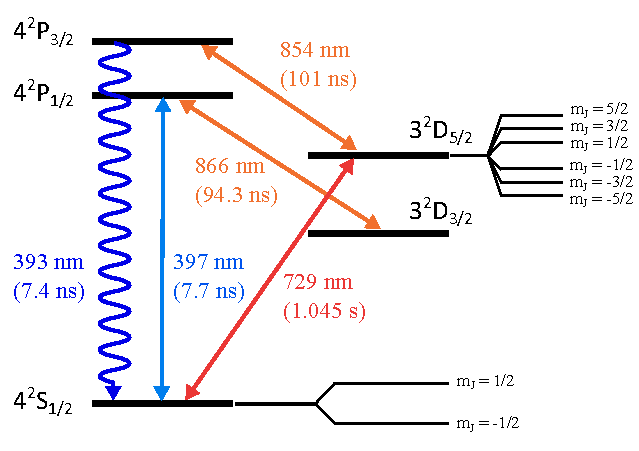
\includegraphics{figures/2/Fig_CaSpec}
        \caption{\label{fig:CaSpec} Level diagram of $^{40}$Ca$^+$ with relevant transitions shown (lifetimes in parentheses). Zeeman splitting is shown for the $S_{1/2}$ and $D_{5/2}$ levels and otherwise omitted. Data from \cite{James98.APB.66.181}.   }
    \end{center}
\end{figure}

The singly charged $^{40}$Ca$^+$ ion is well-researched for many quantum computing and quantum simulation applications \cite{Roos00.Thesis, Häffner2008155, Blatt2012, Schmidt03.Nature.422.408} and as a reference atom in optical atomic clocks \cite{ RevModPhys.87.637, Champenois2004298}. Among its most appealing features is that all of the relevant transitions for ionization, laser cooling, state preparation/detection, qubit operations, and frequency referencing are accessible via solid state laser sources. The level diagram of relevant transitions is shown in Fig. \ref{fig:CaSpec}; the transition wavelengths and lifetimes are summarized in Table \ref{table:CaTransitions} \cite{James98.APB.66.181}. A brief summary of their functions follows. Note that $^{40}$Ca$^+$ has no nuclear spin, and therefore $m_F = m_J$ for all transitions discussed. %The fine structure Zeeman splitting will be of interest to us in the $S_{1/2} \leftrightarrow D_{5/2}$ transition only.  % ; the Land\'{e} factors for these levels is given in Table \ref{table:CaLande} \cite{Roos00.Thesis}.

\begin{table}
\caption{Relevant transition wavelengths and lifetimes in $^{40}$Ca$^+$ \cite{James98.APB.66.181}}
\begin{center}

\begin{tabular}{|c|c|c|c|c|c|}
\hline
  & $S_{1/2} \leftrightarrow P_{1/2}$ & $D_{3/2} \leftrightarrow P_{1/2}$ & $D_{5/2} \leftrightarrow P_{3/2}$ & $S_{1/2} \leftrightarrow P_{3/2}$ & \\ \hline
$\lambda$ & 396.847 & 866.214 & 854.209 & 393.366 & nm \\ \hline
$\tau$ & 7.7 & 94.3 & 101 & 7.4  & ns \\
\hline
\end{tabular}

% table break
\begin{tabular}{c}
\\
\end{tabular}

\begin{tabular}{|c|c|c|}
\hline
 & $S_{1/2} \leftrightarrow D_{5/2}$ & \\ \hline
$\lambda$ & 729.147 & nm \\ \hline
$\tau$ & 1.045 & s \\
\hline 
\end{tabular}
\end{center}
\label{table:CaTransitions}
\end{table}  
%%%%%%%%%%%%
%\begin{table}
%\caption{Relevant Land\'{e} factors \cite{Roos00.Thesis}}
%\begin{center}

%\begin{tabular}{|c|c|c|}
%\hline
 % & $S_{1/2}$ & $D_{5/2}$ \\ \hline
%g_J & 2 & 6/5 \\ 
%\hline
%\end{tabular}
%\end{center}
%\label{table:CaLande}
%\end{table}  
\hfill
\noindent
\begin{flushleft}
\underline{$S_{1/2} \leftrightarrow D_{5/2}$ (729 nm)   }
\end{flushleft}  
This is the primary qubit and reference transition used in $^{40}$Ca$^+$ experiments. It is a quadrupole transition, unlike the rest of those described here (which are dipole), thus it has a suitably long lifetime ($\sim$1 s) for such purposes. Its $\sim$1 Hz natural linewidth also allows for resolution of all the trap secular modes in its spectroscopy. This makes it ideal for resolved sideband cooling, and for any quantum computing or simulation experiments which rely on sideband operations. The secular sidebands in the 729 nm transition are also used to measure the average number of quanta ($\bar{n}$) in their respective modes when the ion is in the Lamb-Dicke regime \cite{Turchette.PRA.61.063418}. 

\begin{figure}[t]
    \begin{center}
        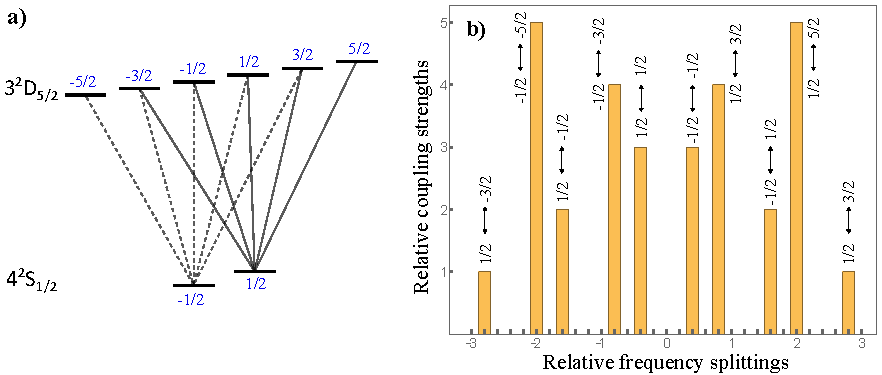
\includegraphics{figures/2/Fig_ZeemanSplits}
        \caption{\label{fig:ZeemanSplits} (a) Allowable transitions of the $S_{1/2} \leftrightarrow D_{5/2}$ quadrupole transition when the ion experiences a non-zero magnetic field. (b) Relative transition coupling strengths vs. relative frequency splittings in an arbitrary magnetic field. The coupling strengths here are dependent on respective Clebsch-Gordan factors. The total span of the frequency splittings is $\sim$ 34 MHz in our experiment, arising from a 4.3 G magnetic field.   }
    \end{center}
\end{figure}

In the presence of a non-zero magnetic field, the electronic states in $^{40}$Ca$^+$ will Zeeman-split into angular momentum states; $S_{1/2}$ and $D_{5/2}$ become $|S_{1/2}, m_J \rangle$ and $|D_{5/2}, m_J\rangle$ (Fig. \ref{fig:ZeemanSplits} (a)). The splittings will be proportional to the applied magnetic field $B$  \cite{Roos00.Thesis}:
\begin{equation}
\Delta E = g_J \ \mu_B \ m_J  B  \text{,}
\end{equation}
where $\mu_B$ is the Bohr magneton and $g_J$ is the Land\'{e} factor for each transition ($g_J = 2\text{,} \ (6/5)}$ for $S_{1/2}$ and $D_{5/2}$, respectively). There will subsequently be ten non-degenerate $|S_{1/2}, m_J \rangle \leftrightarrow |D_{5/2}, m_J\rangle$ transitions which satisfy the quadrupole selection rule $|\Delta m_J| = 0, 1, 2$  (Fig. \ref{fig:ZeemanSplits} (b)). Their relative coupling strengths $\Omega$ depend on respective Clebsch-Gordan factors; they can also be affected by the relative geometry between the magnetic field and the exciting laser's wavevector and polarization (this will be discussed in the next section). In our experiment, a 4.3 G field is sufficient to separate these transitions across a range of approximately 34 MHz. 
\hfill
\noindent
\begin{flushleft}
\underline{$S_{1/2} \leftrightarrow P_{1/2}$ (397 nm)   }
\end{flushleft}
The $S_{1/2} \leftrightarrow P_{1/2}$ transition at 397 nm is used for Doppler cooling, state preparation, and state detection of the ion(s). These functions will be discussed in Secs. 2.5 and 2.6. We detect fluorescence at this wavelength with a photo-multiplier tube (details in Ch. 3).
\hfill
\noindent
\begin{flushleft}
\underline{$D_{3/2} \leftrightarrow P_{1/2}$ (866 nm)   }
\end{flushleft}
Because the $P_{1/2}$ level decays undesirably to the metastable $D_{3/2}$ level approximately 6\% of the time \cite{Roos00.Thesis}, the $D_{3/2} \leftrightarrow P_{1/2}$ transition is continuously driven/repumped by an 866 nm laser in order to avoid population shelving.
\hfill
\noindent
\begin{flushleft}
\underline{$D_{5/2} \leftrightarrow P_{3/2}$ (854 nm)   }
\end{flushleft}
Because the metastable $D_{5/2}$ has a relatively long lifetime on the order of a second, the $D_{5/2} \leftrightarrow P_{3/2}$ transition is driven with an 854 nm laser in order to rapidly depopulate the $D_{5/2}$ state when desired. The short lifetime ($\sim$ 7 ns) of the $P_{3/2}$ state subsequently ensures a rapid return to the $S_{1/2}$ ground state.



\hfill
%%%%%%%%%%%%%
\section{Laser-ion interactions}

We will now discuss the fundamental principles of laser-ion interactions in the approximation of two-level systems. Our treatment follows those in Refs. \cite{Roos00.Thesis, Leibfried03.RMP.75.281}. 

\subsection{Basic interactions}
For a harmonically trapped ion, interacting with a traveling wave laser tuned near to a transition resonance, the corresponding Hamiltonian is
\begin{equation}
\begin{split}
H &= H_0 + H_i \\
H_0 &= \frac{p^2}{2 m} + \frac{1}{2} m \omega_i^2 x^2 + \frac{1}{2} \hbar \omega_0 \sigma_z \\
H_i &= \frac{1}{2} \hbar \Omega (\sigma_+ + \sigma_-) ( e^{i (kx - \nu t + \phi)} + e^{-i (kx - \nu t + \phi)} ) \text{,}	
\end{split}
\label{eq:basicH}
\end{equation}
where $\sigma_z$, $\sigma_+$, $\sigma_-$ are the Pauli spin matricies, $\omega_i$ is the motional frequency of the harmonic potential, $\omega_0$ is the transition frequency, $\Omega$ is the transition coupling strength (or Rabi frequency), $\nu$ is the laser frequency, and $k$ is the laser wavenumber. In this treatment we assume that the both the laser and harmonic oscillations are along the x-axis. The generalization to more dimensions and/or incident angles in the laser is straightforward. 

We can replace various terms in Eq. \ref{eq:basicH} with $a$ and $a^{\dagger}$, the creation and annihilation operators of the harmonic oscillator. Defining the Lamb-Dicke parameter
\begin{equation}
\eta = k \sqrt{ \frac{\hbar}{2 m \omega_i} }
\end{equation}
we get $kx = \eta (a + a^{\dagger})$, and obtain
\begin{equation}
\begin{split}
H_0 &= \hbar \omega_i (a^{\dagger} a + \frac{1}{2} ) + \frac{1}{2} \hbar \omega_0 \sigma_z \\
H_i &= \frac{1}{2} \hbar \Omega (\sigma_+ + \sigma_-) [ e^{i \eta (a + a^{\dagger}) } e^{-i \nu t} e^{i \phi}  +  e^{-i \eta (a + a^{\dagger}) } e^{i \nu t} e^{-i \phi} ]  \text{.}
\end{split}
\end{equation}
Transforming into the interaction picture $H_I = U_0^{\dagger} H U_0$, where $U_0 = exp[-(i / \hbar) H_0 t]$, and discarding the rapidly oscillating terms exp$[\pm i (\nu + \omega_0)]$ (i.e. making the \textit{rotating wave approximation}), we end up with an interaction Hamiltonian of the form 
\begin{equation}
H_I = \frac{1}{2} \hbar \Omega \big( \sigma_+ \ e^{ i \eta [a(t) + a^{\dagger}(t) ] } \ e^{- i \Delta t} \ e^{i \phi}  \big) + H.c. \text{,}
\end{equation}
where $\Delta = \nu - \omega_0$ and $a(t) = a e^{-i \omega_i t}$. This describes coupling between the states $|g, n\rangle$ and $|e, n'\rangle$, where $n$ is the vibrational quantum number and $\hbar (\omega_e - \omega_g) = \hbar \omega_0$. The pairing of the electronic states $|e\rangle$ and $|g\rangle$ with the motional states $|n\rangle$ can also be thought of in the classical sense: the ion, which is oscillating in the trap potential, experiences a frequency-modulated laser in its rest frame which is modulated at the trap frequency. This is the manifestation of secular sidebands in the ion's excitation spectra. If the laser is tuned such that $\nu - \omega_0 \approx m \omega_i$, i.e. onto a sideband, then the transitions $|g,n\rangle \leftrightarrow |e, n+m\rangle$ can be driven. If $\nu - \omega_0 \approx 0$ then the transition $|g,n\rangle \leftrightarrow |e, n\rangle$ will be made with no change in quantum number. We refer to this as the \textit{carrier} transition. Fig. \ref{fig:729spec} shows how these features arise in the $S_{1/2} \leftrightarrow D_{5/2}$ spectroscopy. 

\begin{figure}[t]
    \begin{center}
        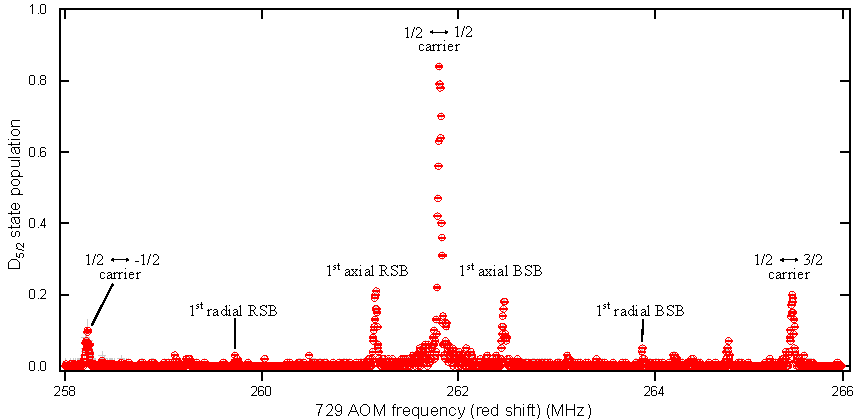
\includegraphics{figures/2/Fig_729spec}
        \caption{\label{fig:729spec} Sample spectroscopy data centered about the $|S_{1/2}, m_J = \frac{1}{2} \rangle \leftrightarrow |D_{5/2}, m_J = \frac{1}{2} \rangle$ carrier transition. Axial and radial sidebands on this transition are labeled. The frequency of the laser is being offset by an acousto-optic modulator (AOM).  }
    \end{center}
\end{figure}

\subsection{Time evolution}
The time evolution of the state $\psi (t) = \Sigma_n ( \ g_n (t) |g, n\rangle + e_{n+m} (t) |e, n + m\rangle \ )$ can be evaluated with the Schr\"{o}dinger equation $ i \hbar \partial_t \psi = H \psi$, which yields a set of coupled differential equations for $g_n (t)$ and $e_{n+m} (t)$. The general solution can be solved analytically as a 2x2 transformation matrix of the initial state vector:     
\begin{equation}
\begin{pmatrix} g_n (t) \\ e_{n+m,n}(t) \end{pmatrix} = T_n \begin{pmatrix} g_n (0) \\ e_{n+m,n} (0) \end{pmatrix} \text{,}
\label{eq:stateEvol}
\end{equation}
with
\begin{equation}
T_n = \begin{pmatrix} e^{-i \frac{\delta t}{2}} \big[ \cos (\frac{f_{n,m} t}{2}) + i \frac{\delta}{f_{m,n}} \sin (\frac{f_{n,m} t}{2}) \big ] & 
- 2 i e^{-i (\frac{\delta t}{2} \ - \frac{\pi |m|}{2} ) } \frac{\Omega_{n+m,m}}{f_{n,m}} \sin (\frac{f_{n,m} t}{2}) \\
 - 2 i e^{i (\frac{\delta t}{2} \ - \frac{\pi |m|}{2} ) } \frac{\Omega_{n+m,m}}{f_{n,m}} \sin (\frac{f_{n,m} t}{2}) &  
 e^{i \frac{\delta t}{2}} \big[ \cos (\frac{f_{n,m} t}{2}) - i \frac{\delta}{f_{m,n}} \sin (\frac{f_{n,m} t}{2}) \big ]
\end{pmatrix}
\text{.}
\label{eq:EvolMatrix}
\end{equation}
Here $\delta = ( \nu - \omega_0 ) - m \omega_i$ is the laser detuning from the $m$'th sideband, 
\begin{equation}
\Omega_{n+m, n} = \Omega \langle n + m | e^{ i \eta [a(t) + a^{\dagger}(t) ] } | n \rangle 
\label{eq:RabiFreq}
\end{equation}
is the scaled coupling strength, and $f_{n,m} = \sqrt{\delta^2 + \Omega_{n+m,n}^2}$ is the detuned frequency. 

We often consider the case with initial conditions $g_n (0) = 1$ and $e_{n+m} (0) = 0$ in Eq. \ref{eq:EvolMatrix}, i.e. the ion prepared initially in its ground state. In this case, the excited state population after a laser-ion interaction time $t$ is 
\begin{equation}
P_{e,n+m} (t) = | e_{n+m} (t) |^2 = \frac{ \Omega_{n+m, n}^2 }{ \delta^2 + \Omega_{n+m, n}^2 } \sin^2 \big( \frac{1}{2} \Omega_{n+m, n} t \big) \text{.}
\label{eq:numstatepop}
\end{equation}
This result characterizes the typical Rabi flopping scenario for driven excitations in a two-level system. 


\subsection{Lamb-Dicke regime approximations}
In the so called Lamb-Dicke regime, defined by ${\eta^2 (2n + 1) \ll 1}$, we can Taylor expand the exponential in Eq. \ref{eq:RabiFreq}:
\begin{equation}
e^{ i \eta [a(t) + a^{\dagger}(t) ] } \approx 1 + i \eta [a(t) + a^{\dagger}(t) ] + \mathcal{O}(\eta^2) \text{.}
\end{equation}
By making this approximation, we find (to lowest orders) explicit definitions of the coupling strengths for the carrier
\begin{equation}
\Omega_{car} = \Omega_{n,n} = \Omega \big[1 - \frac{\eta^2}{2}(1 + 2n) \big] \text{,}
\label{eq:Omega_car}
\end{equation}
the 1st order red sideband
\begin{equation}
\Omega_{rsb} = \Omega_{n-1,n} = \eta \sqrt{n} \ \Omega \ \text{,}
\label{eq:Omega_rsb}
\end{equation}
and the 1st order blue sideband
\begin{equation}
\Omega_{bsb} = \Omega_{n+1,n} = \eta \sqrt{n+1} \ \Omega \ \text{,}
\label{eq:Omega_bsb}
\end{equation}
which can be used in Eq. \ref{eq:numstatepop} for the respective excitations. In our configuration, $\eta \approx 0.07$ for a $(2 \pi) \times 1$ MHz trap frequency. This puts values of $n \lesssim 20$ safely within the Lamb-Dicke regime, which are routinely achievable with Doppler cooling techniques (see Sec. 2.5).


\subsection{Coupling strengths}
The analytical value of $\Omega$ depends on both the transition in question and the geometry of the experimental setup. For the $S_{1/2} \leftrightarrow D_{5/2}$ quadrupole transition, $H_i = \hat{Q} \Delta E(t)$ (i.e. the ion's quadrupole moment is coupled to the gradient of the electric field), and $\Omega$ becomes
\begin{equation}
\Omega =  \bigg| \frac{e E_0}{2 \hbar} \langle S_{1/2}, m_J | (\mathbf{\epsilon \cdot r})(\mathbf{k \cdot r}) | D_{5/2}, m_J' \rangle \bigg| \text{,}
\end{equation}
which is dependent on both the $m_J$ and $m_J'$ values in question (per Fig. \ref{fig:ZeemanSplits} (b)) and the relative geometry between the laser polarization $\mathbf{\epsilon}$, laser wavevector $\mathbf{k}$, and the applied magnetic field $\mathbf{B}$ \cite{James98.APB.66.181, Roos00.Thesis}. A full evaluation can be found in Ref. \cite{Roos00.Thesis}, but for our purposes it will suffice to consider two special cases: 1) $\mathbf{\epsilon}$, $\mathbf{k}$, and $\mathbf{B}$ are all mutually orthogonal, in which case only the $\Delta m = \pm 2$ transitions are coupled, and 2) $\mathbf{k}$ is at an angle $\phi = 45^o$ to $\mathbf{B}$ and $\mathbf{\epsilon}$ is orthogonal to their plane, in which case $\Delta m = 0$ transitions are strongly coupled, $\Delta m = \pm2$ transitions are weakly coupled, and $\Delta m = \pm1$ transitions are not coupled at all. We used the former configuration in the standing wave experiments (Ch. 4) and the latter configuration otherwise. 

In practice is often simplest to determine the coupling strengths empirically. For the $S_{1/2} \leftrightarrow D_{5/2}$ qubit/clock transition in $^{40}$Ca$^+$, a $\sim$ 10 mW resonant laser focused to a $\sim$ 30 $\mu$m waist gives $\Omega \approx$ 3 MHz in our system. This corresponds to a field strength $E_0 \approx 7 \times 10^4$ V/m at the beam center.

%\begin{align*}
%\Omega &=  \bigg| \frac{e E_0}{2 \hbar} \langle S_{1/2}, m_J | (\mathbf{\epsilon \cdot r})(\mathbf{k \cdot r}) | D_{5/2}, m_J' \rangle \bigg| \\
%&= \bigg| \frac{e E_0}{2 \hbar} \langle S_{1/2} || r^2 \mathbf{C}^{(2)} || D_{5/2} \rangle \mathlarger{\sum_{q=-2}^{2}} \begin{pmatrix}1/2 & 2 & 5/2 \\ -m_J & q & m_J' \end{pmatrix} %c_{ij}^{(q)} \epsilon_i n_j \bigg|
%\end{align*}


%%%%%%%%%%%%%%%%%%%%%%%%%%%%%%

\section{Thermal state distributions}

\begin{figure}[t]
    \begin{center}
        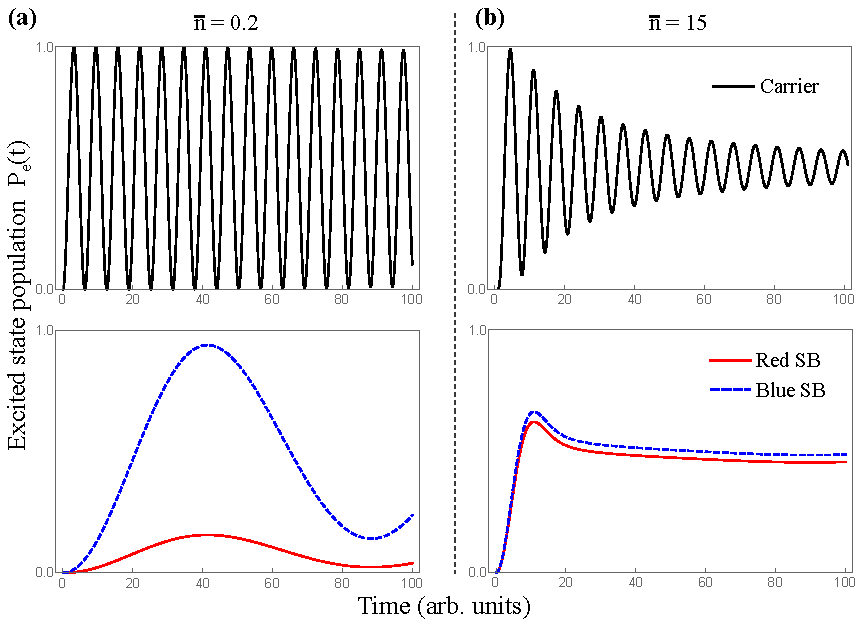
\includegraphics{figures/2/Fig_Flopping}
        \caption{\label{fig:flopping} Simulated carrier (top row) and red/blue sideband (bottom row) Rabi flops for (a) $\bar{n} = 0.2$ and (b) $\bar{n} = 15$, which are representative of our sideband cooled and Doppler cooled ions, respectively. These curves are calculated from Eq. \ref{eq:Pe} and Eqs. \ref{eq:Omega_car} - \ref{eq:Omega_bsb}, with $\delta = 0$. As $\bar{n}$ increases, the population inversion on the carrier loses contrast.  }
    \end{center}
\end{figure}

In practice, a trapped ion does not typically exist in a single number state (or Fock state) $| n \rangle$, but rather in a thermal distribution of number states defined by the probability distribution 
\begin{equation}
P_n (\bar{n}) = \frac{\bar{n}^n}{(\bar{n} + 1)^{n+1}}
\label{eq:Pn}
\end{equation}
where $\bar{n}$ is the average number of quanta in the thermal state \cite{Leibfried03.RMP.75.281}. Therefore, we can generalize Eq. \ref{eq:numstatepop} by summing over all number states. The overall excited state population $P_e (t)$ of the ion becomes 
\begin{equation}
\begin{split}
P_e (t) &= \mathlarger{\sum_{n=0}^{\infty}} \ P_n (\bar{n}) \ P_{e,n+m} (t) \\ 
&= \mathlarger{\sum_{n=0}^{\infty}} P_n (\bar{n}) \frac{ \Omega_{n+m, n}^2 }{ \delta^2 + \Omega_{n+m, n}^2 } \sin^2 \big( \frac{1}{2} \Omega_{n+m, n} t \big)
%(\bar{n}) \frac{ \Omega_{n+m, n}^2 }{ \delta^2 + \Omega_{n+m, n}^2 } \sin^2 \big( \frac{1}{2} \Omega_{n+m, n} t \big)
\label{eq:Pe}
\end{split}
\end{equation}
for a given thermal state characterized by $\bar{n}$. Note that a low value of $\bar{n}$ is necessary in order to achieve the maximum possible contrast in the population transfer (see Fig. \ref{fig:flopping}). Our Doppler cooled ions have $\bar{n} = 10-20$ (depending on various trap factors), which is generally sufficient for good contrast in a single excitation cycle; our sideband cooled ions have $\bar{n} \approx 0.1-0.2$, which is more than ideal. These cooling processes will be described in the next section. Fig. \ref{fig:flopping} shows how Eq. \ref{eq:Pe} evolves for the carrier and 1st order sidebands over this range of $\bar{n}$.


We measure $\bar{n}$ by driving the 1st order red and blue sidebands for a fixed interaction time $t$, and recording the ratio $R_k = (P_e^{rsb} / P_e^{bsb})$. This ratio is independent of $t$, and for thermal states is related to $\bar{n}$ by \cite{Turchette.PRA.61.063418}
\begin{equation}
\bar{n} = \frac{R_k}{1 - R_k} \text{.}
\label{eq:nbar}
\end{equation} 




%%%%%%%%%%%%%%%%%%%%%%%%%%%%%%

\section{Laser cooling techniques} 

We use two different methods of laser cooling to reduce the secular kinetic energy of our ions: Doppler cooling and resolved sideband cooling. We will summarize the basic principles here. Cooling is necessary not only for reaching the Lamb-Dicke regime, but for removing quanta that are continuously gained by the ion due to a variety of heating mechanisms. These include noise in the trap electrodes or external circuitry, noise in the RF drive signal, fluctuating patch potentials on the electrode surfaces, collisions with background atoms, etc \cite{Turchette.PRA.61.063418}. Ions that are not cooled will quickly gain enough energy to overcome the trap potentials, and will be lost.

\subsection{Doppler cooling}
Our description of Doppler cooling follows  Refs. \cite{Doppler, Leibfried03.RMP.75.281}. Doppler cooling is most easily modeled when considering the harmonic pseudopotential in one dimension, $V_{pp}(x) = \frac{1}{2} m \omega_x^2 x^2$\footnote{$V_{pp} = q \Phi_{pp}$.}. Assuming the ion's motion to be classical, then its velocity is given by
\begin{equation}
v(t) = v_0 cos(\omega_x t) \text{.}
\end{equation}
If we excite the ion to a state with an average lifetime $\tau$ that is much less than an oscillation period, then the ion's velocity is effectively constant throughout the cycle of absorption and spontaneous emission. This allows the average radiation pressure exerted by the exciting laser to be modeled as a continuous force dependent on the ion's velocity. 

In typical conditions, the average force can be linearized in $v$:
\begin{equation}
F_{ave} \approx F_0 (1 + \kappa v) \text{,}
\end{equation}
where $F_0 \propto \hbar k$, \footnote{If the exciting laser is at an angle $\theta$ to the ion's oscillation axis, then $k$ is simply replaced by $k \cos (\theta)$.} and $\kappa \propto \Delta = \nu - \omega_0$, with $\Delta$ being the laser detuning from resonance as before. The average change in energy of the ion over many oscillation periods can therefore be described as
%\begin{equation}
%\kappa = \frac{ 8 k \Delta / \Gamma^2 }{1 + 2( \Omega / \Gamma)^2 + (2 \Delta / \Gamma)^2 } \text{.}
%\end{equation}
%Here, $\Delta = \nu - \omega_0$ is the laser detuning from transition resonance, $\Gamma$ is the transition decay rate (or linewidth), and $\Omega$ is the on-resonance coupling strength. 
\begin{equation}
\frac{d E}{d t} = \langle F_{ave} v \rangle = F_0 \langle v \rangle + F_0 \kappa \langle v^2 \rangle = F_0 \kappa \langle v^2 \rangle \text{,}
\end{equation}
since $\langle v(t) \rangle = 0$. Because $\kappa \propto \Delta$, $( d E / d t )$ will be negative when $\Delta < 0$, and the ion will subsequently be cooled. At the same time, there will be some amount of heating present due to recoil from the emission cycles. Cooling will continue until equilibrium is reached between these two processes, which places a limit on the degree of cooling achievable. This limit is reached when the laser detuning is
\begin{equation}
\Delta = - \frac{\Gamma}{2} \sqrt{1 + 2 (\Omega / \Gamma)^2} \approx - \frac{\Gamma}{2} \text{,}
\end{equation}
where $\Gamma$ is the transition decay rate (or linewidth), $\Omega$ is the on-resonance coupling strength, and $\Gamma \gg \Omega$, generally. In practice the transition can be power-broadened beyond its natural linewidth $\Gamma$ by an intense enough laser, in which case it is sufficient to set $\Delta$ to approximately the FWHM value.

In our system we use the 397 nm laser to Doppler cool on the $S_{1/2} \rightarrow P_{1/2}$ transition, which has $\tau = 7.7$ ns and a corresponding linewidth $\Gamma \approx$ 20 MHz. We red-detune the laser by 10 MHz to achieve maximum cooling, which produces $\bar{n} = 10-20$ for a single ion (depending on trap factors such as stray fields). Doppler cooling is performed continuously when the ion is idle, simply by virtue of the laser being switched on. When cooling immediately before, during, or after an experiment, we use pulses that are $100 - 400$ $\mu$s in duration (depending on available beam power).   

\subsection{Sideband cooling}
To cool the ion(s) beyond the Doppler limit we must use resolved sideband cooling techniques. Detailed descriptions of these methods can be found in Refs. \cite{Leibfried03.RMP.75.281, Cirac92.PRA.46.2668, PhysRevA.20.1521, RevModPhys.58.699}. Sideband cooling is performed on transitions where $\Gamma \ll \omega_i$, i.e. when the transition linewidth is sufficiently narrow for the sidebands to be resolved. In this case, we can excite the transition directly on a red sideband (i.e. $|g,n\rangle \rightarrow |e, n+m\rangle$ for $m<0$) and subsequently reduce the vibrational quantum number. The 1st order red sideband ($m = -1$) is generally used since it couples most strongly. Each successive excitation on the 1st order red sideband removes an additional quanta, until the ion approaches its motional ground state. At this point, the average number of motional quanta $\bar{n}$ is approximately
\begin{equation}
\bar{n} \approx \frac{\Gamma^2}{4 \omega_i^2} \ \text{,} %\bigg[ \bigg(\frac{\tilde{\eta}}{\eta}\bigg)^2 + \frac{1}{4} \bigg] \text{,}
\end{equation}
where $\eta$ and $\tilde{\eta}$ are Lamb-Dicke factors associated with absorption and emission processes, respectively. %The bracketed term is of order unity, therefore $\bar{n} \ll 1$ since $\omega_i \ll \Gamma$. 
This is equivalent to the ion being in the ground state $|0\rangle$ with a probability very close to 1. 

When the red sideband transition is allowed to decay naturally via spontaneous emission, the cooling rate $R_n$ depends on both the decay rate $\Gamma$ and the red sideband coupling strength $\Omega_{rsb} = \eta \sqrt{n} \ \Omega$:
\begin{equation}
R_n = \Gamma \ \frac{(\eta \sqrt{n} \ \Omega)^2}{2(\eta \sqrt{n} \ \Omega)^2 + \Gamma^2} \text{.}
\end{equation}
This can be very slow, given that $\Gamma$ is often on the order of Hz, $\eta \ll 1$, and $n$ is continuously decreasing. It is possible to speed up this process by coupling the excited state to an auxiliary state with a much shorter lifetime. The effective decay rate $\tilde{\Gamma}$ becomes
\begin{equation}
\tilde{\Gamma} = \frac{\Omega_{aux}^2}{(\Gamma_{aux} + \Gamma)^2 + 4 \Delta_{aux}^2} \ \Gamma_{aux}
\end{equation}
and is adjustable via the coupling laser's power and detuning $\Delta_{aux}$. 

In our system we sideband cool on the 1st order red sideband of the $S_{1/2} \rightarrow D_{5/2}$ transition ($\Gamma \approx 1$ Hz), which is excited by the appropriately tuned 729 nm laser. Beginning with a Doppler cooled ion, we drive the $S_{1/2} \rightarrow D_{5/2}$ sideband on resonance for a time period $T_n = \pi / (\eta \sqrt{n} \Omega)$, assuming $n \approx 15$ intially. We then use 854 nm light to couple the $D_{5/2}$ state to the auxiliary $ P_{3/2}$ state, which subsequently decays back to the $S_{1/2}$ ground state on the order of nanoseconds. A $5-10$ $\mu$s pulse of 854 nm light at modest intensities is sufficient to clear the $D_{5/2}$ population. We repeat these steps 2 or 3 times since the population inversion on the red sideband transition is never complete (see Fig. \ref{fig:flopping}). The entire process is then repeated with an updated value of $T_n$, until we achieve measured values of $\bar{n} = 0.1-0.2$. 



%Every absorption/excitation event exerts a change in momentum $\Delta p = \hbar k \cos(\theta)$ upon the ion, where $\theta$ is the angle between the laser and the motional axis (for simplicity, we will assume $\theta = 0$). The rate of absorption-emission cycles is equal to $\Gamma \rho_{ee}$, where $\Gamma$ is the decay rate (or linewidth) of the transition and $\rho_{ee} = \langle e | \hat{\rho} | e \rangle$ is the density matrix element corresponding to the excited state probability. In this case, $\rho_{ee}$ is defined as
%\begin{equation}
%\rho_{ee} = \frac{s/2}{1 + s + [ 2 (\Delta - \mathbf{k \cdot v}) / \Gamma ]^2} \text{,}
%\end{equation} 
%where $s = 




%%%%%%%%%%%%%%%%%%%%%%%%%%%%%%%%%
\section{State preparation and detection}

\begin{figure}[t]
    \begin{center}
        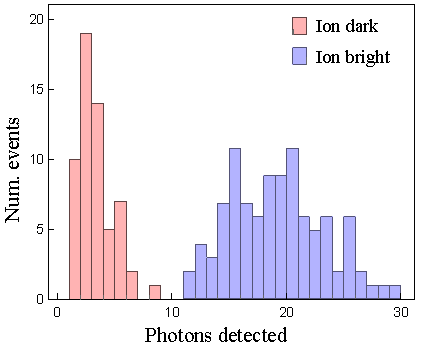
\includegraphics{figures/2/Fig_histograms}
        \caption{\label{fig:histograms} Example histograms for a ``dark'' and ``bright'' ion, which are either non-fluorescing or fluorescing, respectively, represented by the number of photons detected in a given detection time. So long as the respective distributions are distinguishable, then the number of photons detected during a detection event can be correlated to the ion's state (i.e. $S_{1/2}$ or $D_{5/2}$) at the time of measurement.}
    \end{center}
\end{figure}

During Doppler cooling, the spontaneous decay of the $P_{3/2}$ state will populate the $|S_{1/2}, m_J = \frac{1}{2} \rangle$ and $|S_{1/2}, m_J = -\frac{1}{2} \rangle$ states equally on average. Subsequently, any coherent excitation to a $|D_{5/2}, m_J \rangle$ state will achieve $\approx$ 50\% population inversion at best. To selectively prepare ion(s) in a single ground state Zeeman level, we pulse them with circularly polarized 397 nm light that is co-axial to the applied magnetic field. This couples only the $|S_{1/2}, m_J = \frac{1}{2} \rangle$ or $|S_{1/2}, m_J = -\frac{1}{2} \rangle$ level to the $P_{3/2}$ state, depending on whether the light is $\sigma_-$ or $\sigma_+$ polarized, and will depopulate that particular state over many cycles. We can state prepare either $m_J$ level to between 95-99 \% population (limited by the polarization optics and exact beam angle relative to $\mathbf{B})$. 

We also require a reliable method of measuring the ion's final state, i.e. measuring $P_e(t)$ in Eq. \ref{eq:Pe}, after performing coherent operations on the $S_{1/2} \rightarrow D_{5/2}$ transition. Pulsing the ion with the 397 nm laser projects it into into either the $S_{1/2}$ or $D_{5/2}$ state, with outcome probabilities $1 - P_e(t)$ and $P_e(t)$ respectively. The ion will then either fluoresce on the $S_{1/2} \leftrightarrow P_{1/2}$ transition in the former outcome, or remain dark in the latter. This is the so-called electron shelving method \cite{Roos00.Thesis, Leibfried03.RMP.75.281}. As long as the fluorescing ion produces enough photon counts on a detector to be distinguishable from dark/background (see Fig. \ref{fig:histograms}), then this process can be repeated until a suitable histogram of measurement outcomes is accumulated, providing a measured value of $P_e(t)$.  



%%%%%%%%%%%%%%%%%%%%%%%%%%%%%%%%%%
\section{Micromotion effects and compensation}

All of the theory and experimental details discussed here assume the ion is located on the RF null, and therefore neglect micromotion. If the ion is pushed off of the RF null by stray electric fields, or otherwise, then there can be significant issues. In particular, the linewidth of the 397 nm $S_{1/2} \leftrightarrow P_{1/2}$ transition becomes broadened and ``flattened'' as the micromotion modulation increases, since $\Gamma$ is on the order of $\Omega_{RF}$ in this case. This effectively cripples Doppler cooling, and makes state detection impossible since there is no longer a discernible resonance peak to distinguish a fluorescing ion from a dark one (i.e. the histograms in Fig. \ref{fig:histograms} cannot be discerned). By tuning the 397 nm laser to the red micromotion sideband (not the blue, since Doppler heating would occur when $\Delta > 0)$ and adjusting the ion's position until fluorescence is minimized, we can compensate for micromotion in the plane of the laser. Other methods of detecting and minimizing minimization exist, such as measuring average ion displacements as a function of trap potentials, or monitoring the amplitude of resolved sidebands, or using parametric excitations \cite{Berkeland98.JAP.83.5025, doi:10.1063/1.4930037}, but for our purposes the method described is sufficient.

Even when we make these compensations, non-trivial micromotion could still be occurring in the direction orthogonal to the plane of the laser. This can be problematic when measuring spectroscopy on a transition where $\Gamma \ll \Omega_{RF}$, as there will exist micromotion sidebands that are significantly removed in frequency relative to the transition's linewidth and the spread of its angular momentum states and secular sidebands. If the transition resonance frequencies are not already known, it can be easy to confuse a set of micromotion sideband spectra with the carrier spectra--a fact we learned during the course of these experiments. Deliberately displacing the ion from the RF null is a way to distinguish these features--if the coupling strengths get stronger, then they are micromotion sidebands. 